\section{Deleting Data Packages}

You can remove any data package that you have created—both from the
network and/or your local machine—by choosing to open or search for data
packages, and then selecting the package you wish to delete from the
listed packages. Right-click the data package and select ``Delete'' from
the drop-down menu (\autoref{fig:open-dp-delete}). You cannot delete
packages that other users have created unless they have granted you
special permissions. Also, deleting packages from the network does not
technically delete them: deleted packages are archived and excluded from
searches.

\begin{figure}
  \centering
    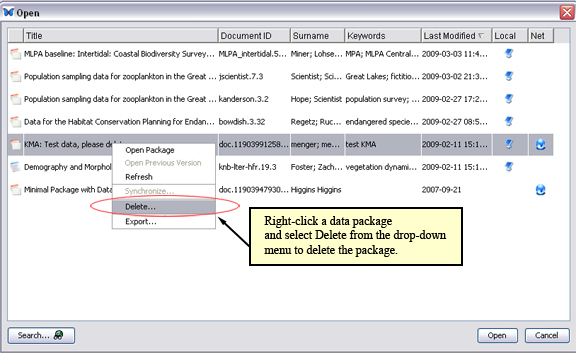
\includegraphics[width=0.7\textwidth]{images/open-dp-delete.jpg}
  \caption{Deleting a data package.}
  \label{fig:open-dp-delete}
\end{figure}

Before deleting the data package, Morpho asks for confirmation. Choose
whether to delete a local copy, a network copy, or both local and
network copies using the check boxes on the confirmation screen.
